Med udgangspunkt i domænemodellen udviklet i arkitekturfasen er der udviklet applikationsmodeller for hver computer i systemet. Dette giver overblik over de funktionaliteter som skal implementeres på de forskellige platforme.

Applikationsmodellen består af at beskrive hvordan information fordeles i hvert UC. Dette opnåes med tre diagram typer. Sekvensdiagrammer som viser hvordan information bevæger sig sekventielt igennem systemets klasser, et klassediagram som sammenfatter de metoder og relationer som er fundet i sekvensdiagrammet og et tilstandsmaskinediagram som viser et systems forskellige tilstande. Det sidste er udeladt da det ikke er aktuelt for det opbyggede system.

%
% Applikationsmodel for PC
%
\subsection{Applikationsmodel for PC (JC)}

Ud fra domænemodellen og de forskellige UC er der oprettet sekvens diagrammer for hver use case (UC4 og UC7 undtaget, UC4 fordi den er utrolig simpel og UC7 fordi den refererer til UC8) Sekvensdiagrammet for UC2 Aktiver kan ses på nedenstående gifur \ref{lab:Sekvensdiagram UC2}. Resten af sekvensdiagrammerne kan ses i projektdokumentationen.

\begin{figure}[htbp] \centering
{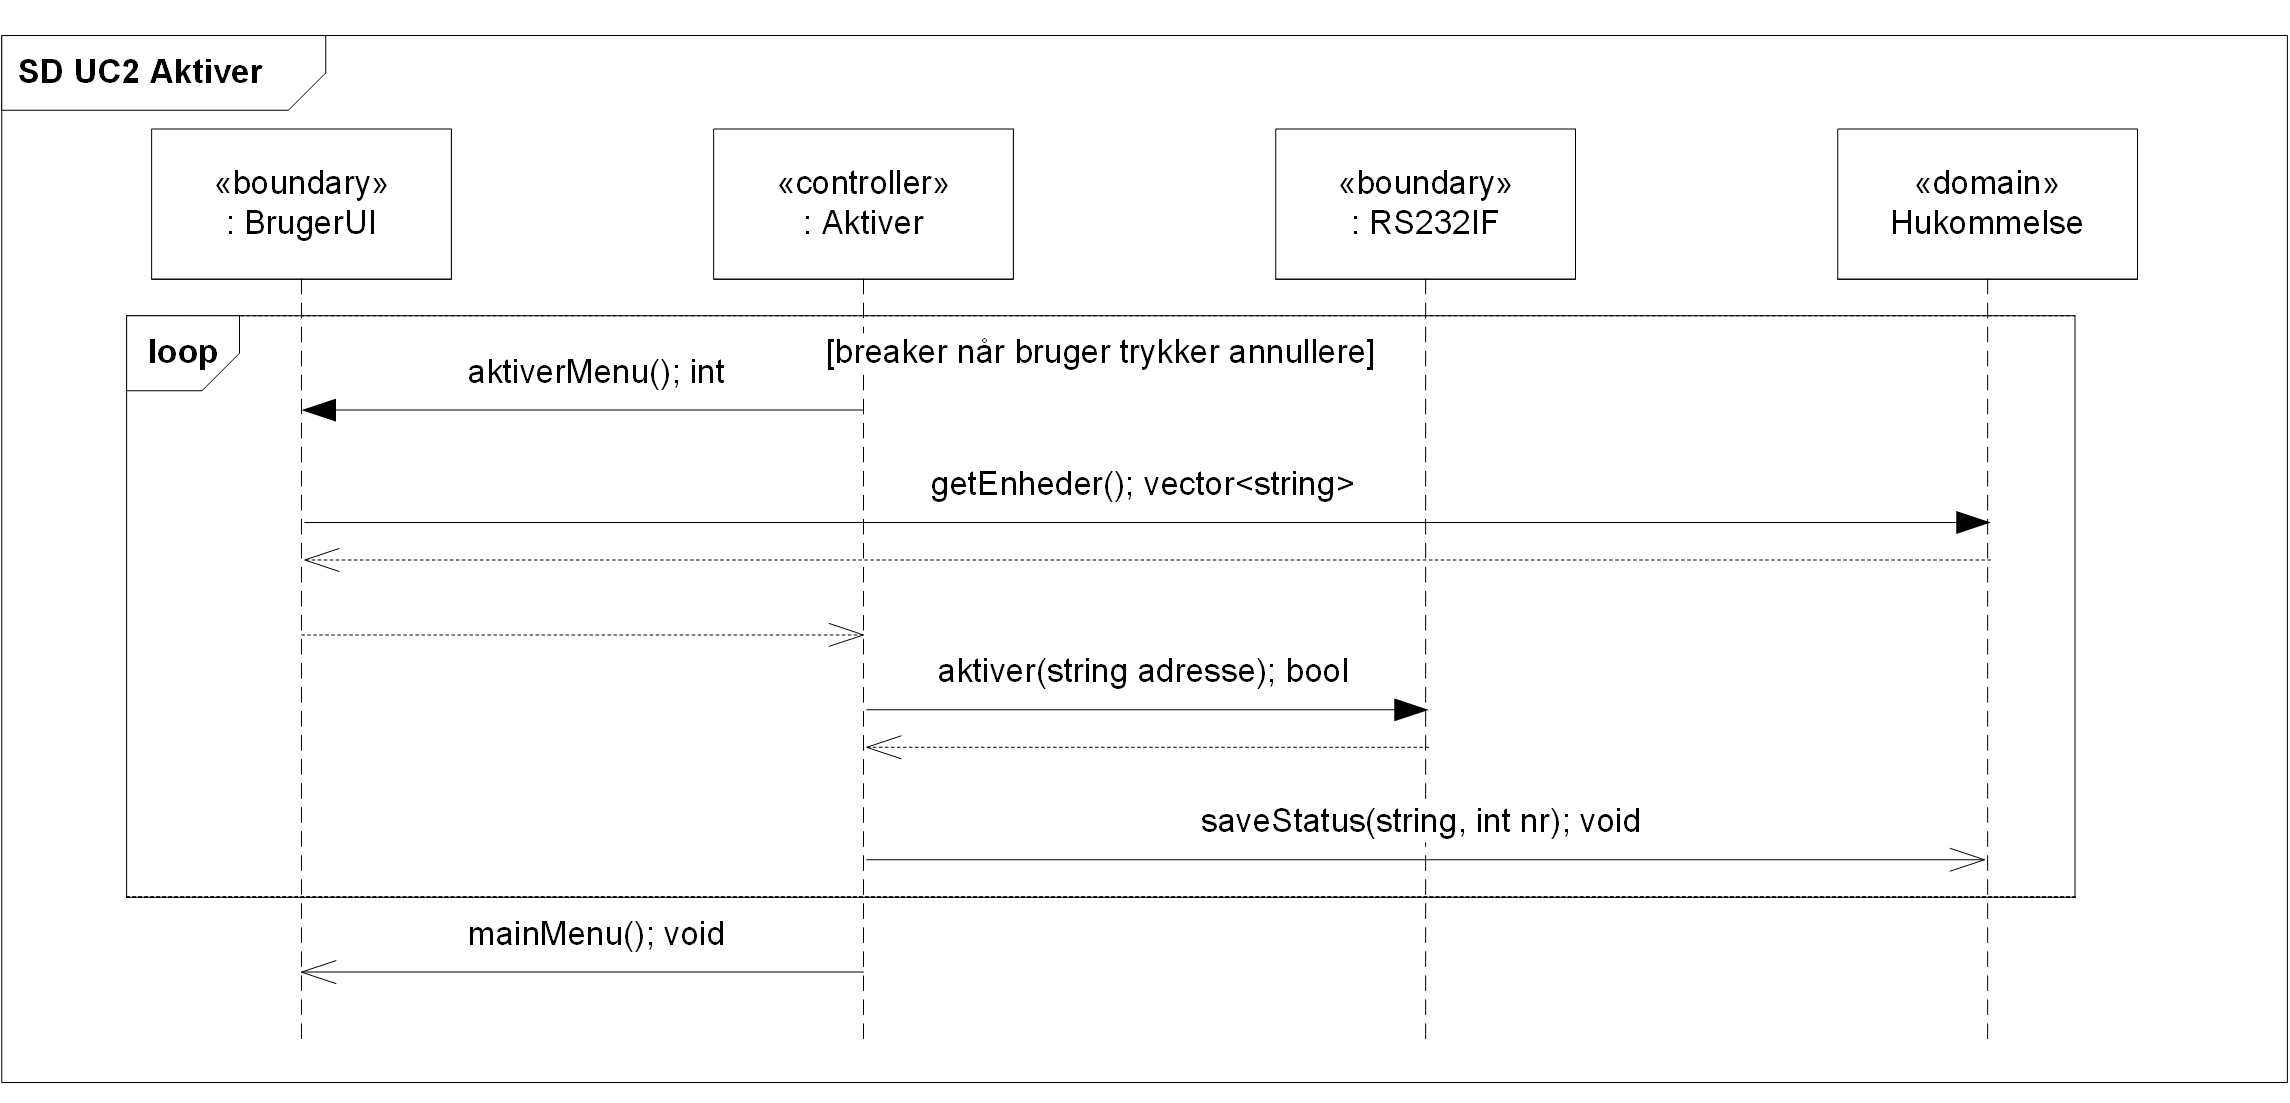
\includegraphics[width=\textwidth]{billeder/uml/PC_UC2}}
\caption{Sekvensdiagram UC2}
\label{lab:Sekvensdiagram UC2}
\end{figure}

Efter at alle sekvensdiagrammerne er lavet har vi alle vores konceptuelle klasser med metoder som vi nu kan overføre til et klassediagram som ses på figur \ref{lab: PC klasse diagram}.

\clearpage
\begin{figure}[htbp] \centering
{\includegraphics[width=\textwidth]{billeder/uml/PC_class}}
\caption{PC klasse diagram}
\label{lab: PC klasse diagram}
\end{figure}

Når det konceptuelle klassediagram er lavet, kan man arbejde  videre med et statisk klassediagram samt tilhørende klassebeskrivelser. Herefter kan designet begynde. 

%
% Applikationsmodel for CSS-hovedenhed
%
\subsection{Applikationsmodel for CSS-hovedenhed (BS)}
Med udgangspunkt i systemdomænemodellen, figur \ref{lab:domainmodel}, er de konceptuelle klasser for CSS-hovedenheden udledt. 

Med dette udgangspunkt laves der sekvensdiagrammer for hvert UC. Disse er vist i figur \ref{fig:CSS_hovedenhed_sd}. De viser hvordan metodekald imellem de konceptuelle klasser fra domænemodellen og giver et overblik over den basale funktionalitet. Her er kun medtaget UC1. Se projektdokumentationen\footnote{\textbf{Reference til sidetal!!!}} for resten.

\begin{figure}[!htb]
     \centering
     { 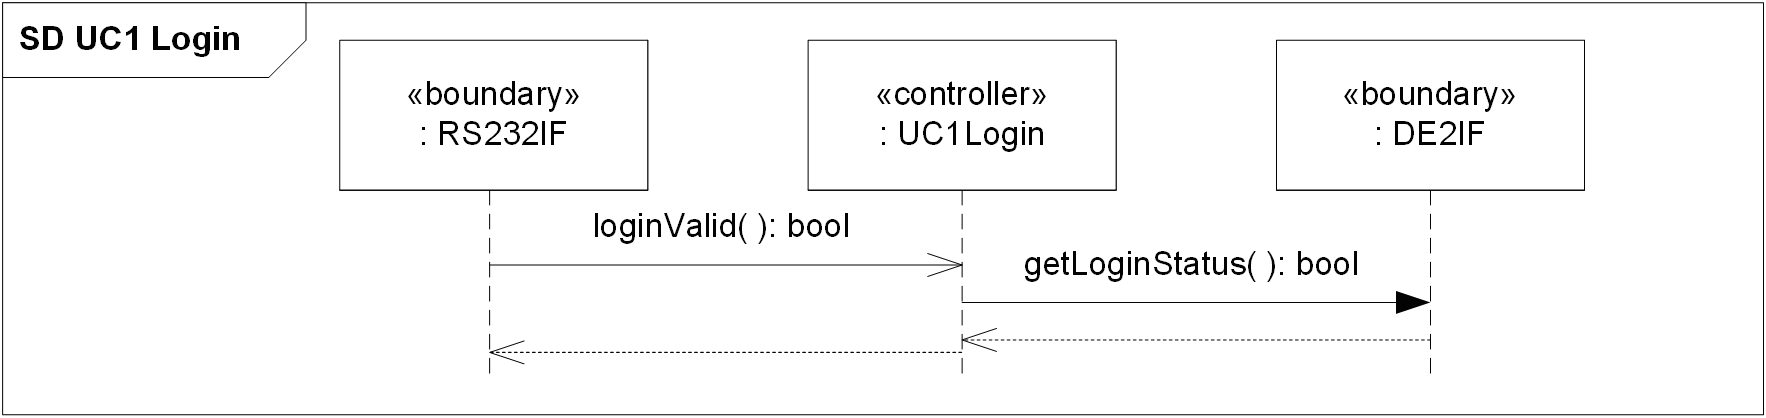
\includegraphics[width=0.9\textwidth]{Billeder/UML/CSS_hovedenhed_SD}}
     \caption{Sekvensdiagram for CSS-hovedenhed}
     \label{fig:CSS_hovedenhed_sd}
\end{figure}

Dette resulterer i et klassediagram med grundfunktionaliteterne, se figure \ref{fig:CSS_hovedenhed_class}. Denne bruges under implementeringen og ender ud i et statisk klassediagram som beskriver det endelige program med alle hjælpemetoder.

\begin{figure}[!htb]
     \centering
     { 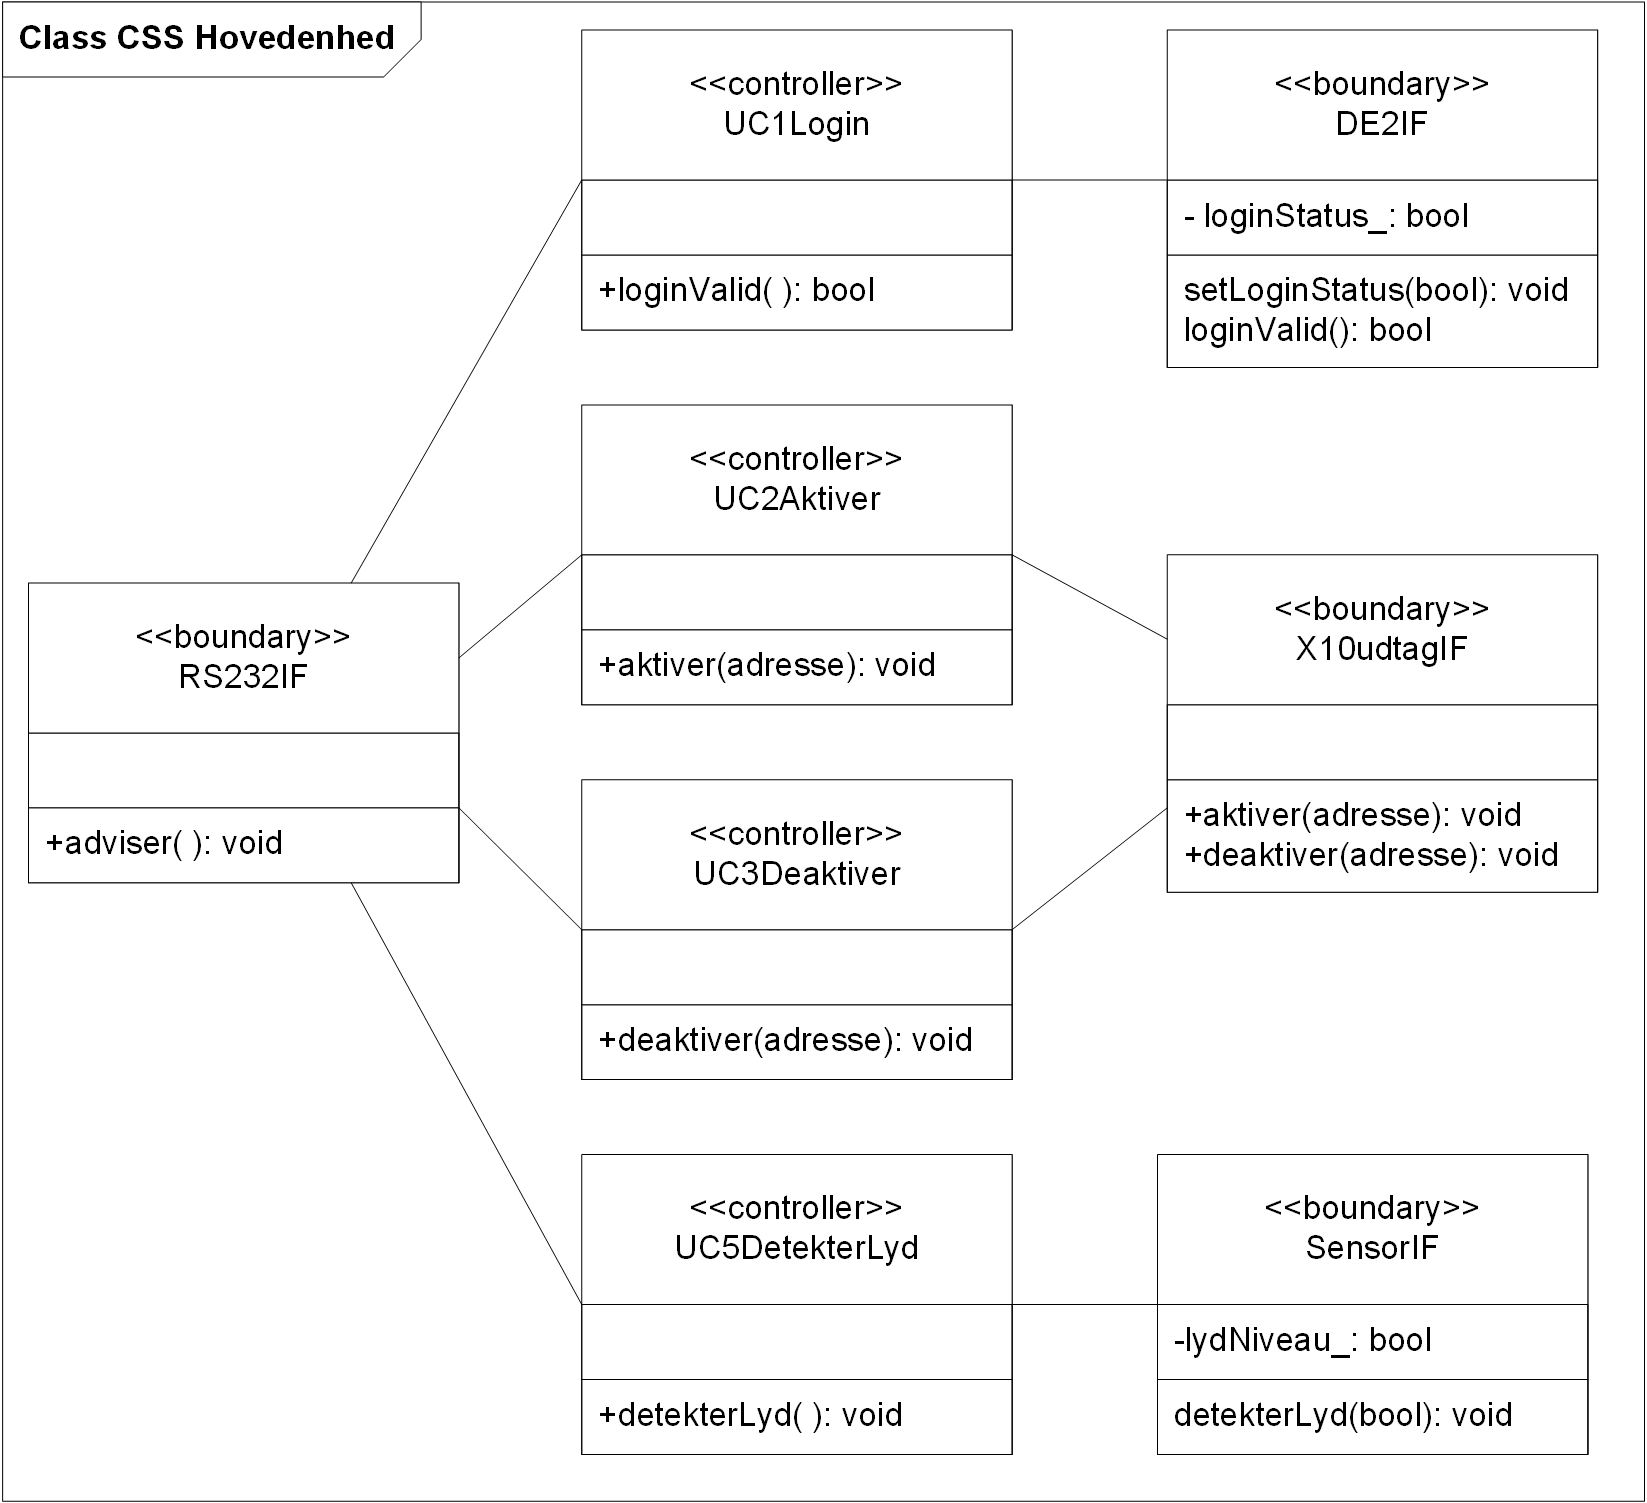
\includegraphics[width=0.9\textwidth]{Billeder/UML/CSS_hovedenhed_Class}}
     \caption{Klassediagram for CSS-hovedenhed}
     \label{fig:CSS_hovedenhed_class}
\end{figure}

Efter denne analyse er der et klart overblik til implementeringsfasen.

%
% Applikationsmodel for X10-udtag
%
\subsection{Applikationsmodel for X10-udtag (BS)}
Først er der lavet en detaljeret domænemodel for X10 udtaget. Denne er vist i figur \ref{fig:X10_udtag_domaenemodel}. Denne laves ved at gennemgå UC beskrivelserne og finde de ting som har indflydelse på netop denne del af systemet.

\begin{figure}[!htb]
     \centering
     { 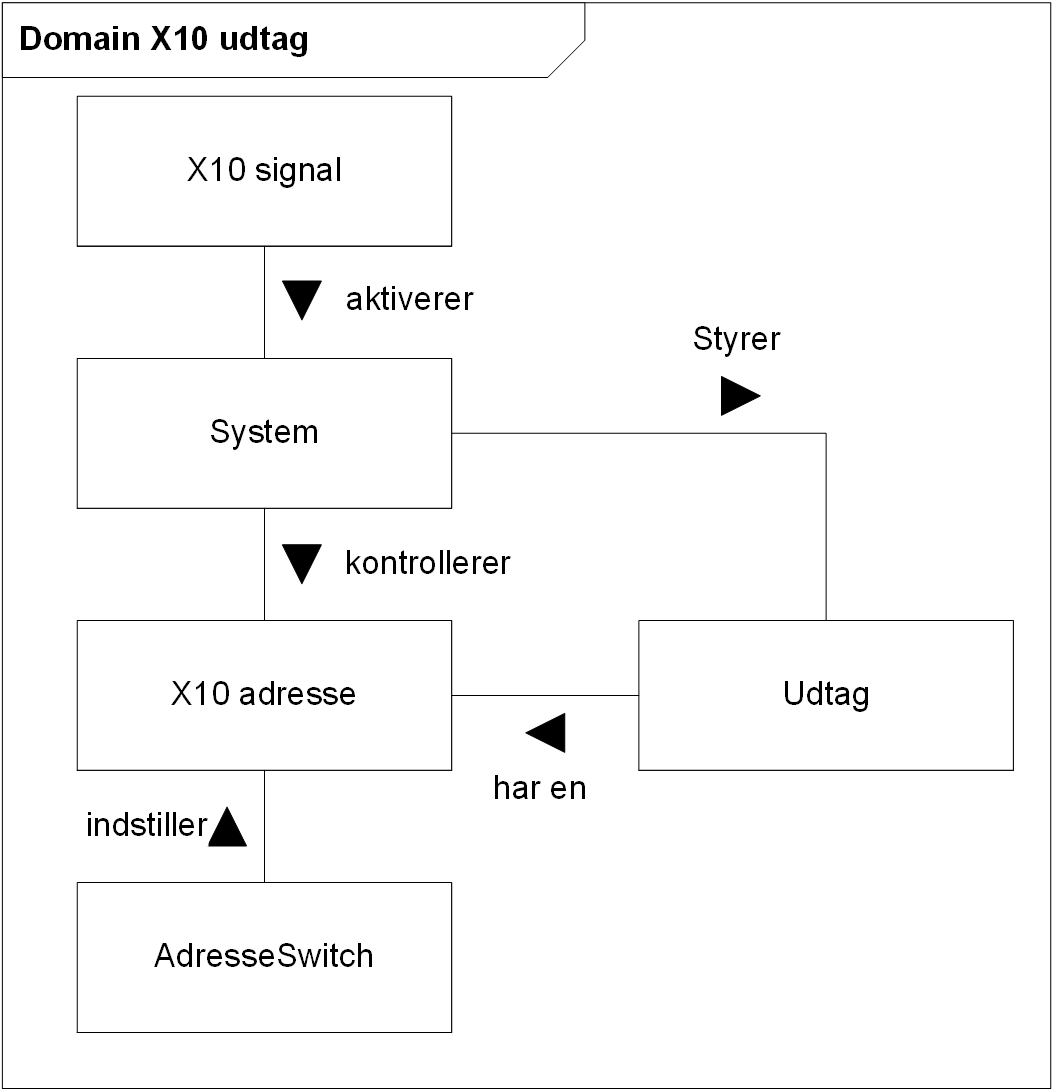
\includegraphics[width=0.7\textwidth]{Billeder/UML/X10_modtager_Domain}}
     \caption{Domænemodel for X10-udtag}
     \label{fig:X10_udtag_domaenemodel}
\end{figure}

Med dette udgangspunkt laves der sekvensdiagrammer for hvert UC. Disse er vist i figur \ref{fig:X10_udtag_sd}. De viser metodekald i mellem de konceptuelle klasser og giver et overblik over den basale funktionalitet. Her er kun medtaget UC2 Aktiver. Se projektdokumentationen\footnote{\textbf{SE SIDETAL!}} for resten.

\begin{figure}[!htb]
     \centering
     { 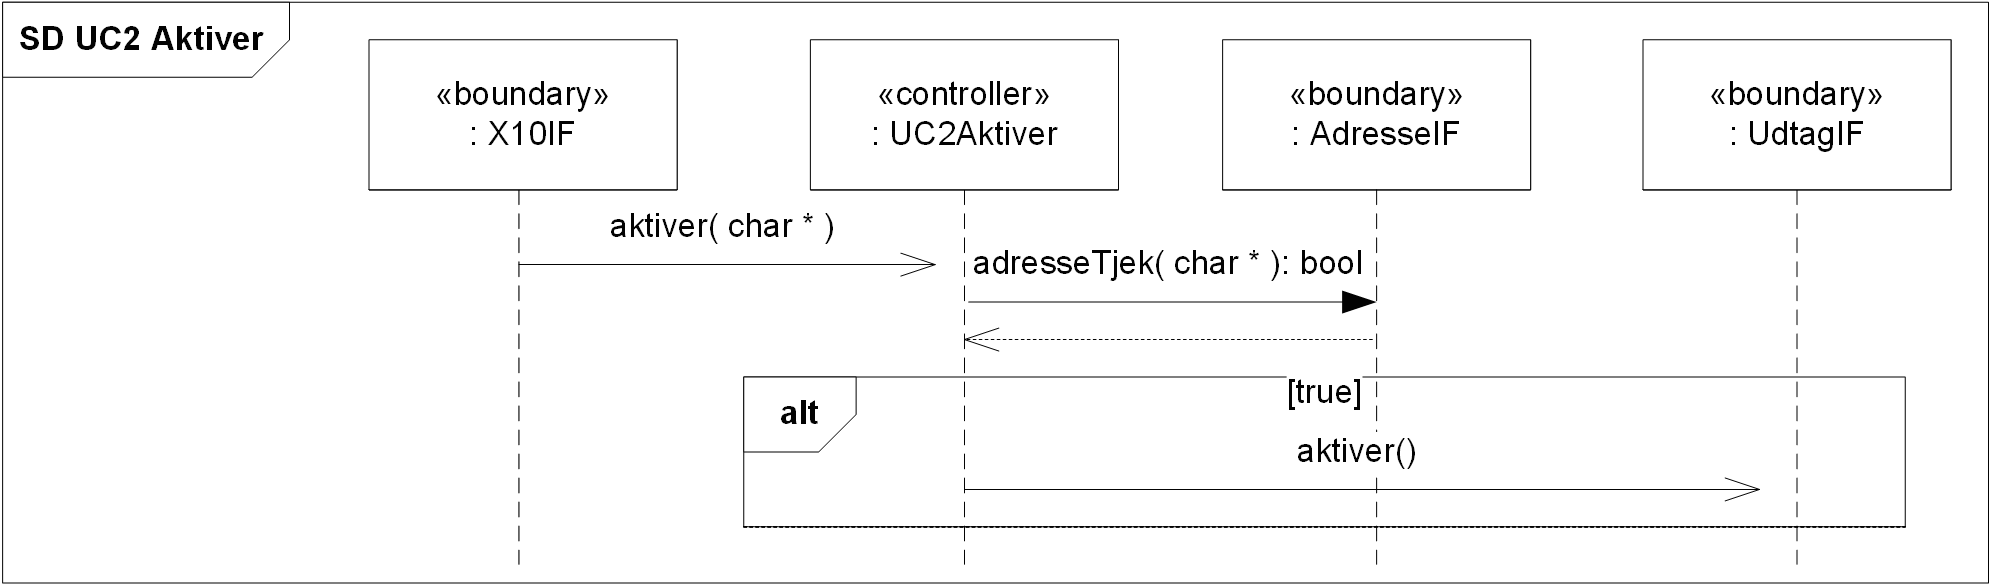
\includegraphics[width=0.9\textwidth]{Billeder/UML/X10_modtager_SD}}
     \caption{Sekvensdiagram for X10-udtag}
     \label{fig:X10_udtag_sd}
\end{figure}

Dette resulterer i et klassediagram med grundfunktionaliteten beskrevet, se figure \ref{fig:X10_udtag_class}. Denne bruges under implementeringen og ender ud i et statisk klassediagram som beskriver det endelige program med alle hjælpemetoder.

\begin{figure}[!htb]
     \centering
     { 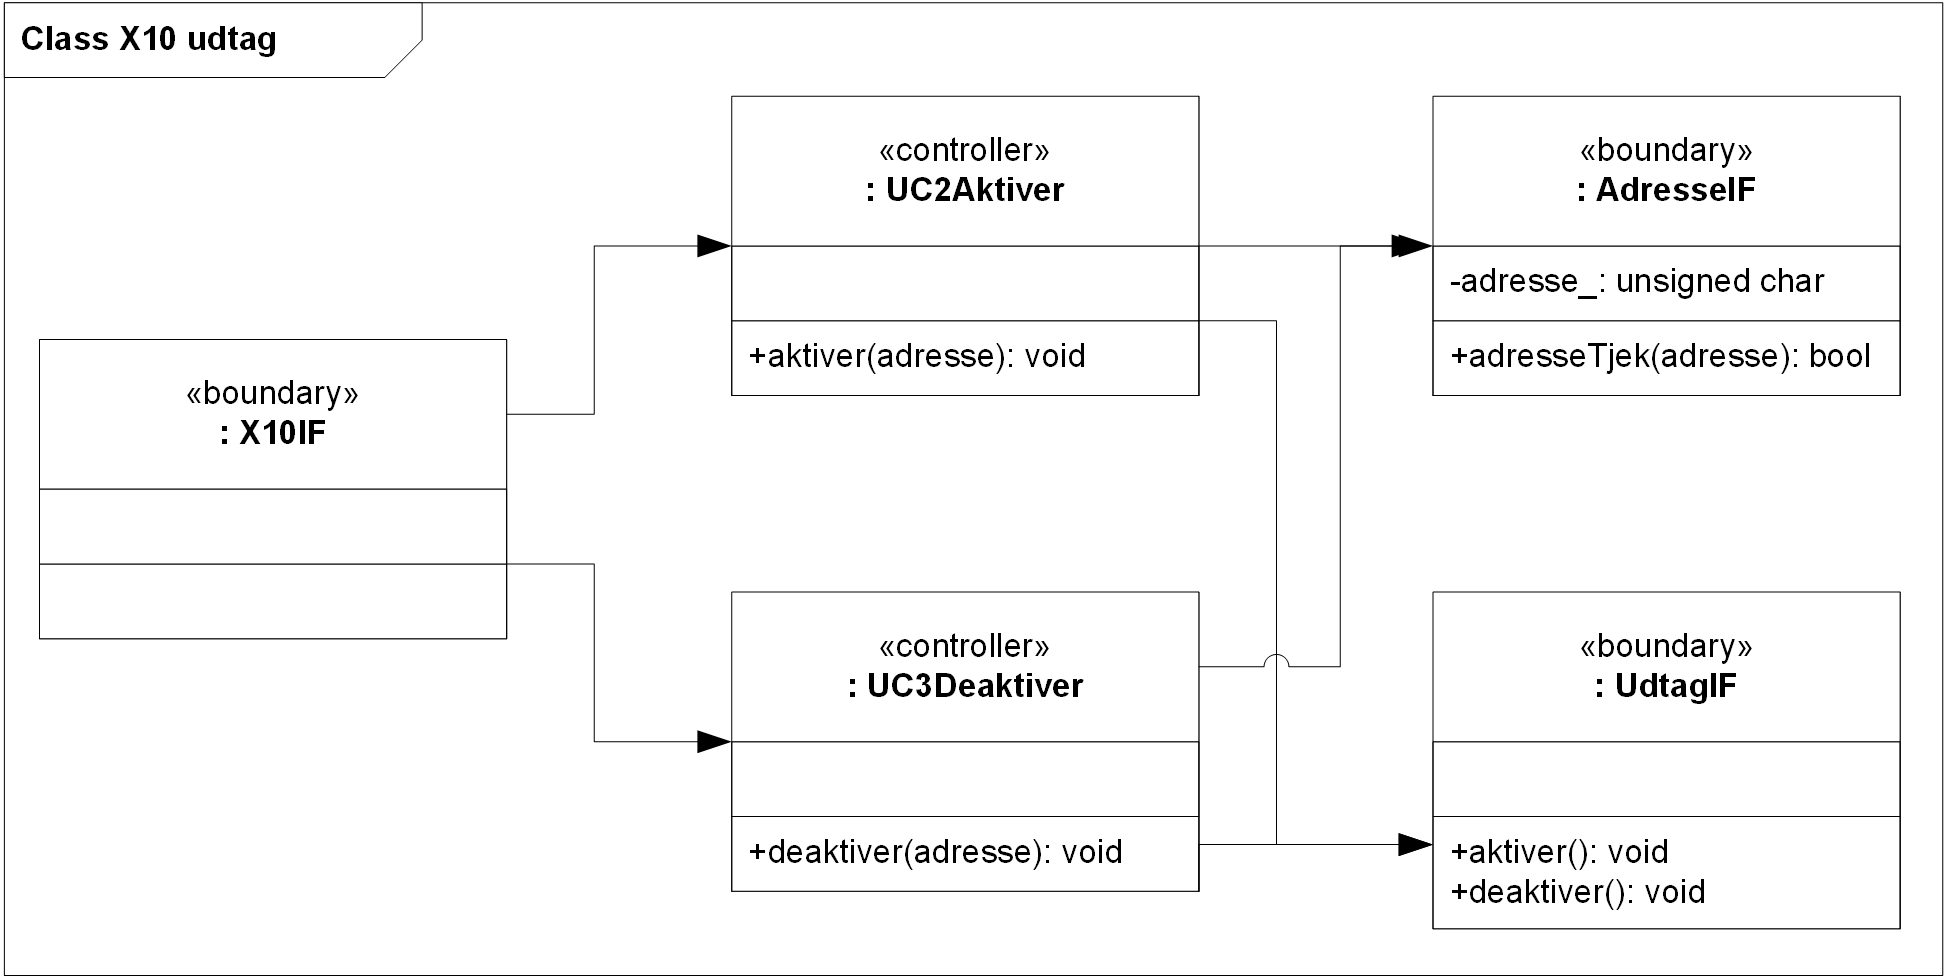
\includegraphics[width=0.9\textwidth]{Billeder/UML/X10_modtager_Class}}
     \caption{Klassediagram for X10-udtag}
     \label{fig:X10_udtag_class}
\end{figure}

Denne analyse af funktionalitet giver et klart overblik til implementeringsfasen.